\chapter{Introduction}
\label{ch:introduction}
As far back as 400 BC, humans pondered the fundamental makeup of the natural world. The Greek philosopher Democritus proposed the notion that matter cannot be infinitely divisible. Thus, there must exist a smallest, indivisible particle, which he termed the 'atom' (from Greek \textit{atomos} meaning 'indivisible'). Although this idea was not empirically tested but derived from philosophical musings, it marked the inception of the quest for a fundamental understanding of the universe.

More than 2000 years later, in 1808, the chemist John Dalton refined Democritus's idea by introducing the concept of elements. Each element was seen as a distinct, indivisible atom differing in mass and size. This refined model enabled Dalton to account for the apparent conservation of mass.

In the late 19$^\text{th}$ century, physicist Sir Joseph John Thomson developed an atomic model portraying atoms as positively charged spheres containing lighter, negatively charged particles known as electrons. The atom as a concept was no longer the smallest, most fundamental particle. Thomson's model was derived from experiments utilising a hot, radiating cathode emitting electrons, thus explaining the observed cathode electron beam.

In 1911, Ernest Rutherford conducted an experiment using an $\alpha$-particle beam directed at a thin gold foil. The results suggested that the majority of an atom's mass is concentrated in a very small volume – the positively charged nucleus – surrounded by negatively charged electrons orbiting in mostly empty space.

Two years later, in 1913, Niels Bohr refined the model further, likening the motion of electrons around the nucleus to planets orbiting the sun. He proposed that electrons move in circular orbits without emitting radiation, with orbit radii restricted to specific quantised values, marking the inception of quantum mechanics.

Electrons can transition between orbits by emitting or absorbing photons of quantised energies, thus explaining the photoelectric effect. In 1916, Arnold Sommerfeld expanded the Bohr model, permitting elliptical orbits and providing an explanation for the presence of closely spaced spectral lines.

In 1926, Werner Heisenberg and Erwin Schrödinger independently developed a mathematical framework for quantum mechanics. The requirement that electrons adhere to Schrödinger's equation led to the concept of atomic orbitals – regions in space with a high probability of containing electrons, subject to specific selection rules.

While the concept of an atomic nucleus was first proposed by Rutherford, it was initially thought to consist solely of positively charged protons. However, this model was expanded in 1932 by James Chadwick, who introduced neutral particles, neutrons, as constituents of the nucleus.

Today, research into the fundamental structure of nature continues, with particle physics superseding nuclear physics. The contemporary aim of particle physics is to develop a comprehensive understanding of fundamental phenomena, centred around formulating and expanding upon the Standard Model of particle physics, which stands as the most successful description of the fundamental nature of the universe.


\chapter{The Standard Model of Particle Physics}
\label{ch:standard_model}

The Standard Model of particle physics (SM) stands as the most triumphant framework to date in understanding the fundamental particles and their interactions. It encompasses all known elementary particles along with their antiparticles, and three out of the four recognised fundamental forces: the strong, weak, and electromagnetic forces. Notably, gravity remains beyond the scope of the SM.

The SM is a renormalisable quantum field theory characterised by an internal SU(3)$\otimes$SU(2)$\otimes$U(1) gauge symmetry. The SU(3) group symmetry elucidates the strong interactions, stemming from quantum chromodynamics (QCD) \cite{qcd}, while the SU(2)$\otimes$U(1) group symmetry corresponds to the electroweak interactions. The latter entails the unification of the electromagnetic force, originating from quantum electrodynamics (QED) \cite{qed01, qed02, qed03}, and the weak force, stemming from quantum flavour dynamics (QFD) \cite{qft}.

Incorporated into the electroweak interaction in 1967, the Brout-Englert-Higgs mechanism introduces a quantum Higgs-field \cite{higgs_mechanism_1, higgs_mechanism_2, higgs_mechanism_3}. This mechanism instigates spontaneous symmetry breaking within the SU(2)$\otimes$U(1) symmetry. Initially, all bosons are massless, yet this symmetry breaking results in bosons interacting with the Higgs-field to become massive. Fermions, too, acquire their masses via interaction with the Higgs-field. The massive gauge bosons of the electroweak interaction are denoted as the \zwboson. Furthermore, one of the degrees of freedom introduced by the Higgs-field which is not defined via the Brout-Englert-Higgs mechanism, manifests as the scalar Higgs-boson $H$ \cite{higgs_mechanism_1}.

Despite the SM's commendable precision in predicting most observations, certain phenomena elude its fundamental explanations. Notably, neutrino oscillations \cite{neutrino_oscillation} exemplify this shortfall, delineating flavour-changing neutrinos. This oscillation necessitates at least two massive neutrinos, while the SM posits all neutrinos as massless. Consequently, the SM fails to account for neutrino oscillations. Another enigma is dark matter \cite{dark_matter}. The measured rotational velocities of vast spiral galaxies necessitate significantly more mass than visible matter provides. These astronomical observations indicate the presence of a stable form of matter that eludes electromagnetic interaction, rendering it invisible. No particle within the SM can explain these measurements.


\section{Characteristics of the Top Quark}
\section{sec:theory_top}
The discovery of the top ($t$) quark took place in 1995 at \fermilab through the collaborative efforts of the \dzero \cite{top_production01} and \cdf \cite{top_production02} experiments. With a mass of $m_t=172.76\pm0.30,\text{GeV}$ \cite{top_mass}, the top quark is acknowledged as the most massive among all known quarks. Its exceedingly brief lifespan is approximately $tau_t\approx5\cdot10^{-25},\text{s}$ \cite{top_mass}. Upon decaying through the weak interaction, the top quark decays into a \wboson and a down-type quark which then undergoes hadronisation. The likelihood of decaying into a specific down-type quark is determined by the corresponding CKM-matrix element \cite{ckm_matrix}. Given that the CKM-matrix predominantly features vanishing off-diagonal elements, the primary decay mode for top quarks involves transitioning into \bquarks. Subsequently, the \wboson undergoes further decay, either into a charged lepton and neutrino, yielding one observable jet originating from the \bquark alongside a detectable lepton, or into a quark-antiquark pair, resulting in the production of three detectable jets.

Generating \tquarks necessitates significant energies owing to the mass of the \tquark. Such energies are attainable in hadron colliders. Figure~\ref{fig:production_ttz_ttw} illustrates two exemplar processes for \tquark production within \ttbar processes. Each of the two \tquarks decays as previously described. Thus, the observed signal is contingent upon the decay mode of the \wboson.


\section{Effective Field Theory}
\label{sec:theory_eft}
For examining phenomena beyond the Standard Model, one can adopt an Effective Field Theory (EFT) framework like the Standard-Model Effective Field Theory (SM-EFT) \cite{eft_operatorlist}. This approach assumes that the current Standard Model serves as a practical low-energy approximation, valid for interactions up to an energy scale $\Lambda$. It can be expanded using higher-dimensional interactions \cite{eft_introduction}. The transition to the Standard Model occurs through the decoupling of heavy particles at energies greater than $\Lambda$. Thus, higher-dimensional operators $Q$, suppressed by powers of $\Lambda$, are utilised in a perturbation expansion \cite{eft_introduction}.
\begin{align}
\mathcal{L}\text{SM-EFT} = \mathcal{L}\text{SM} + \frac{1}{\Lambda}\sum_{k}C_k^{(5)}Q_k^{(5)} + \frac{1}{\Lambda^2}\sum_{k}C_k^{(6)}Q_k^{(6)} + \mathcal{O}\left(\frac{1}{\Lambda^3}\right);.\label{eq:SM-EFT}
\end{align}
In this expansion, $\mathcal{L}_\text{SM}$ denotes the standard SM Lagrangian, $Q_k^{(n)}$ represents the $n$-dimensional interaction operators, and $C_k^{(n)}$ are their corresponding Wilson coefficients.

For a deeper understanding of \ttbarZ and \ttbarW production, it's valuable to scrutinise their pertinent operators. Given that the \zboson combines the $W^0$ and $B$ bosons originating from the Brout-Englert-Higgs mechanism, the operator \optZ for the $tZ$ coupling is expressed as \cite{higgs_mechanism_1}
\begin{align}
Q_\text{tZ} &= \cos(\Theta_W)Q_\text{tW} - \sin(\Theta_W)Q_\text{tB};.\label{eq:OparatortZ}
\end{align}
Therefore, the operators for the $tW$ and the $tB$ couplings, along with their complex coefficients \ctW and \ctB, are particularly pertinent for this analysis \cite{eft_operatorlist}. To quantify sensitivity, the separation power
\begin{align}
S &= \frac{1}{2}\sum_\text{Bins}\frac{\left(\text{EFT}_i-\text{SM}_i\right)^2}{\text{EFT}_i+\text{SM}_i}\label{eq:SeparationPower}
\end{align}
is employed. The expression within the summation is computed for each bin based on a given normalised distribution. Here, $\text{SM}$ denotes the Standard Model prediction, and $\text{EFT}$ incorporates a specific variation on one or multiple Wilson coefficients as shown in Equation~\ref{eq:SM-EFT}. Investigations concerning the sensitivity of various variables for these coefficients are summarised in Chapter~\ref{ch:eft_sensitivity}.


\chapter{Experimental Setup}
\label{ch:experimental_setup}
To collect data on \ttbarZ and \ttbarW events, a high-energy particle collider is indispensable. Additionally, a setup for signal detection and suitable reconstruction algorithms are required.

The Large Hadron Collider (\lhc), spanning 27 kilometres, operates as a proton-proton collider. During Run~I, it achieved a centre-of-mass energy of approximately 7-8 TeV, rising to 13 TeV in Run~II \cite{lhc2}. For Run~III, an anticipated centre-of-mass energy of 13.6 TeV is projected \cite{lhc_run3}. These high-energy collisions yield multiple particles, including \tquarks, which subsequently decay into additional particles. Detecting these events necessitates a calibrated detector system capable of measuring particle properties such as charge, momentum, and energy. Moreover, event reconstruction from measured signals involves employing various algorithms to reconstruct, for instance, particle trajectories and collision vertices.

The \atlas-detector \cite{atlas} serves as a versatile particle detector comprising distinct layers designed to detect various particles. These layers are arranged in concentric cylinders around the beam axis. Through tracking measurements and energy deposition of decay products, the initial particles can be reconstructed. Figure~\ref{fig:atlas} illustrates a schematic representation of these detector layers. Each layer is described below.

\begin{figure}[t]
    \centering
    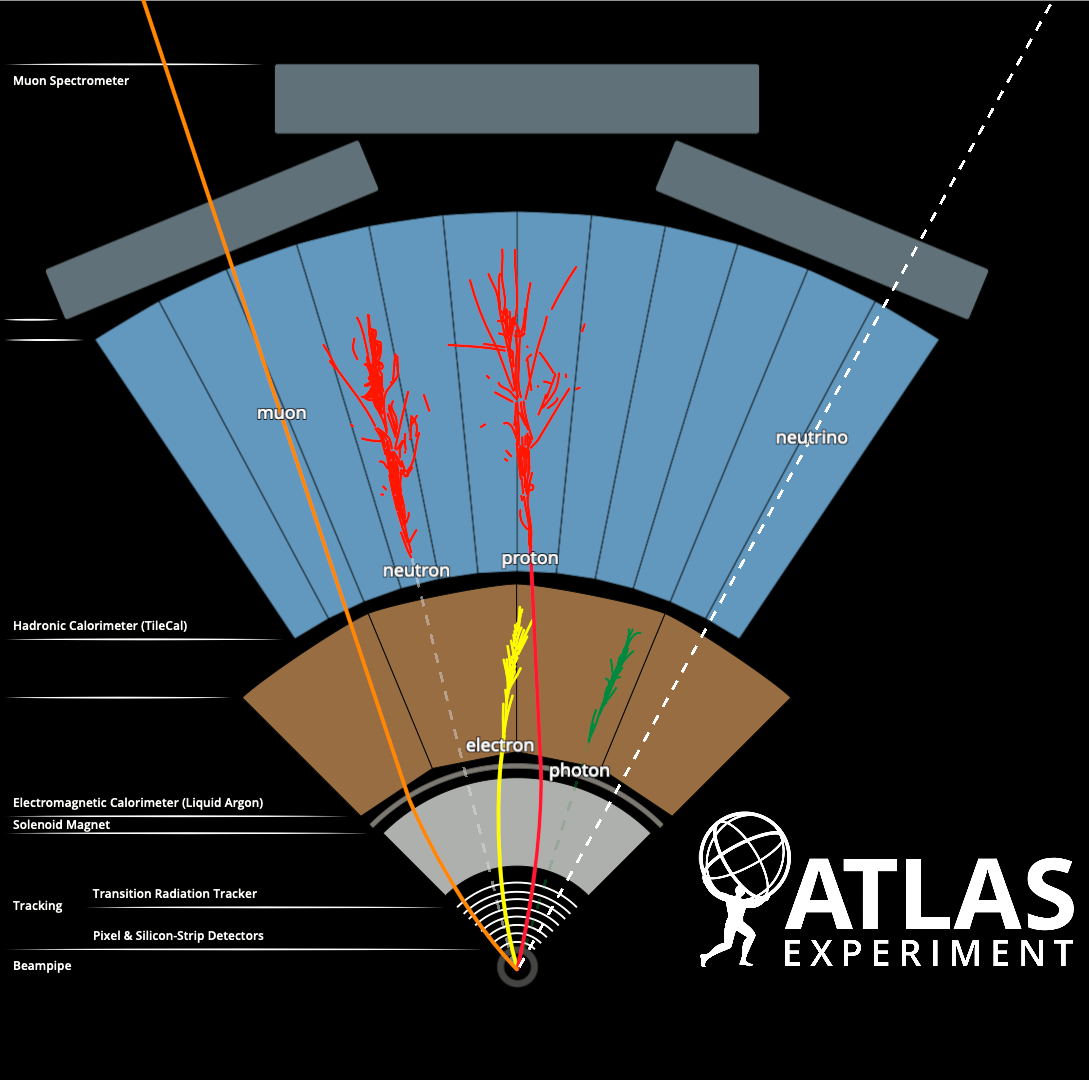
\includegraphics[width=.61\textwidth]{figures/atlas/atlas3.png}
    \caption{Cross-section of the concentric layers within the \atlas Detector (\copyright{} \cern)}
    \label{fig:atlas}
\end{figure}

\section*{The Inner Detector}
The Inner Detector is tasked with precisely measuring the tracks of various charged particles. A 2 T magnetic field, generated by a central solenoid, causes the movement of charged particles to deflect via the Lorentz force. By measuring the curvature, precise momentum measurements and particle track reconstruction are achieved. This tracking system is vital for $b$-tagging, enabling the identification of secondary vertices, indicative of $b$-jets \cite{atlas}. Given the high particle density near the collision point, high-precision measurements utilise Pixel, Strip, and Transition Radiation Trackers.

The Pixel Tracker, constructed from silicon to withstand collision radiation, detects tracks near the collision point using small Pixel-modules \cite{atlas}. The Semiconductor Strip Tracker (SCT) comprises longer strips, enhancing tracking with larger scale measurements.

The Transition Radiation Tracker (TRT) consists of thin polyimide straws filled with a gas mixture \cite{atlas}. While offering a lower resolution, these straws provide a cost-effective means to cover a larger volume, contributing to precise measurements. The TRT aids in distinguishing electrons $e^\pm$ from charged pions $\pi^\pm$.

\section*{The Calorimeters}
As depicted in Figure~\ref{fig:atlas}, the calorimeters envelop the Inner Detector and the solenoid magnet. Generally, they measure particle energy by halting their motion. The \atlas-detector utilises electromagnetic and hadronic calorimeters, both sampling calorimeters comprising an absorber material inducing particle showers and an active medium for signal measurement \cite{atlas_calorimeter}.

The electromagnetic calorimeter detects particles interacting electromagnetically, with charged particles and photons generating electromagnetic showers. This facilitates reconstruction of initial particles, offering precise energy measurement and deposition location. Constructed with Lead as the absorber and liquid Argon as the active medium, it provides accurate measurements \cite{atlas_calorimeter}.

The hadronic calorimeter absorbs particles passing through the electromagnetic calorimeter that interact via the strong force. Hadronic showers produced may yield additional electromagnetic sub-showers, complicating reconstruction and reducing precision. Comprising steel as the absorber and plastic scintillating tiles, it fulfils its role effectively \cite{atlas_calorimeter}.

\section*{The Muon Spectrometer}
Serving as the outermost layer, the Muon Spectrometer employs a similar approach to the Inner Detector to measure muon momentum, typically undetected by the Inner Detector and Calorimeter. It comprises four subsystems \cite{atlas}.

For muon triggering and coordinate measurement, Resistive Plate Chambers (RPC) and Thin Gap Chambers (TGC) are deployed across different detector regions. Additionally, Cathode Strip Chambers (CSC) offer precise coordinate measurements at the detector ends. Monitored Drift Tubes (MDT) track muon trajectories' curvature. Outer toroidal magnets generate the magnetic field responsible for muon deflection \cite{atlas}.


\chapter{Current Status}
\label{ch:current_status}

\chapter{Outlook}
\label{ch:outlook}

\section{SPANet}
\section{ttH}
\section{Neutrino Weighting}
